\documentclass[11pt, twoside, pdftex]{article}

% This includes all the settings that we should use for the document
% This includes all the settings that we should use for the document
\newcommand{\PDFTitle}{Using the DE-Series ADC Controller}
\newcommand{\commonPath}{../../Common}
\newcommand{\datePublished}{Mar 2022}

\newcommand{\versnum}{21.1} %version number quartus/AMP
\newcommand{\quartusname}{Quartus\textsuperscript{\textregistered} Prime}	
\newcommand{\textBar}{For \quartusname{} \versnum{}}
\newcommand{\thisyear}{2022 } %for copyright
\newcommand{\company}{FPGAcademy.org}
\newcommand{\longteamname}{FPGAcademy.org}
\newcommand{\teamname}{FPGAcademy}
\newcommand{\website}{FPGAcademy.org}

\newcommand{\productAcronym}{AMP}
\newcommand{\productNameShort}{Monitor Program}

\newcommand{\productNameMedTM}{Monitor Program}
\newcommand{\productNameMed}{Monitor Program}

%\newcommand{\headerLogoFilePath}[1]{#1/FPGAcademy.png}



\setlength\topmargin{-0.25in}
\setlength\headheight{0in}
\setlength\headsep{0.35in}
\setlength\textheight{8.5in}
\setlength\textwidth{7in}
\setlength\oddsidemargin{-0.25in}
\setlength\evensidemargin{-0.25in}
\setlength\parindent{0.25in}
\setlength\parskip{0in} 

\pdfpagewidth 8.5in
\pdfpageheight 11in

% listings is a package that supports encapsulating source code in LaTeX conveniently

\usepackage{listings}
% add support for graphics
\usepackage{graphicx}
\usepackage[usenames, dvipsnames]{color}

\def\expandparam\lstinputlisting[#1]#2{\edef\tmp{\noexpand\lstinputlisting[#1]{#2}}\tmp}

\widowpenalty 10000
\clubpenalty 10000

%%%%%%%%%%%%%%%%%%%% Source Code Formatting %%%%%%%%%%%%%%%%%%%%
\definecolor{globalCommentColour}{rgb}{0.588,0.588,0.588}

%%%%%%%%%%%%%%%%%%%%%%%%%%%%%%%%%%%%%%%%%%%%%%%%%%%%
% Defining a NiosII ASM highlighter for lstlisting
\lstdefinelanguage[NiosII]{Assembler} {
 	morekeywords={add, addi, and, andhi, andi, beq, bge, bgeu, bgt, bgtu, ble,  bleu, blt, bltu, bne, br, break,% 
 	bret, call, callr, cmpeq, cmpeqi, cmpge, cmpgei, cmpgeu, cmpgeui, cmpgt, cmpgti, cmpgtu, cmpgtui, cmple,%
 	cmplei, cmpleu, cmpleui, cmplt, cmplti, cmpltu, cmpltui, cmpne, cmpnei, custom, div, divu, eret, flushd,%
 	flushda, flushi, flushp, initd, initda, initi, jmp, jmpi, ldb, ldbio, ldbu, ldbuio, ldh, ldhio, ldhu, ldhuio,%
 	ldw, ldwio, mov, movhi, movi, movia, movui, mul, muli, mulxss, mulxsu, mulxuu, nextpc, nop, nor, or, orhi, ori,%
 	rdctl, rdprs, ret, rol, roli, ror, sll, slli, sra, srai, srl, srli, stb, stbio, sth, sthio, stw, stwio,%
 	sub, subi, sync, trap, wrctl, wrtcl, wrprs, xor, xori, xorhi, xori},% 	
 	morekeywords=[2]{.abort, .ABORT, .align, .app-file, .ascii, .asciz, .balign, .byte, .comm, .data, .def,%
 	.desc, .dim, .double, .eject, .else, .end, .endef, .endif, .equ, .equiv, .err, .extern, .file, .fill, .float,%
 	.global, .globl, .hword, .ident, .if, .include, .int, .irp, .irpc, .lcomm, .lflags, .line, .linkonce, .ln,%
 	.list, .long, .macro, .mri, .nolist, .octa, .org, .p2align, .psize, .quad, .rept, .sbttl, .scl, .section,%
 	.set, .short, .single, .size, .sleb128, .skip, .space, .stadb, .stabn, .stabs, .string, .symver, .tag,%
 	.text, .title, .type, .val, .uleb128, .word},% 	
 	morekeywords=[3]{et, bt, gp, sp, fp, ea, sstatus, ra, pc, status, estatus, bstatus, ienable, ipending, cpuid,%
 	exception, pteaddr, tlbacc, tlbmisc, eccinj, badaddr, config, mpubase, mpuacc},% 	
 	sensitive=t,%
 	alsoletter=.,%
	morestring=[b]",%
 	morecomment=[s]{/*}{*/},%
 	morecomment=[l]\#,%
   }[keywords,comments,strings]
   
   %% NOTE: morekeywords=[2] are GNU directives.
   
   \definecolor{niosInstructionColour}{rgb}{0.000,0.608,0.000}
   \definecolor{niosDirectiveColour}{rgb}{0.000,0.000,0.902}
   \definecolor{niosSpecialRegColour}{rgb}{0.000,0.000,0.000}
   \definecolor{niosStringColour}{rgb}{0.808,0.482,0.000}
   
   %% NOTE: To make bold use: =\bfseries\color{<colour>}
   \lstdefinestyle{defaultNiosStyle} {
   language=[NiosII]{Assembler},
   stringstyle=\color{niosStringColour},
   keywordstyle=\color{niosInstructionColour},
   keywordstyle=[2]\color{niosDirectiveColour},
   keywordstyle=[3]\itshape\color{niosSpecialRegColour}
   }
%%%%%%%%%%%%%%%%%%%%%%%%%%%%%%%%%%%%%%%%%%%%%%%%%%%%

%%%%%%%%%%%%%%%%%%%%%%%%%%%%%%%%%%%%%%%%%%%%%%%%%%%%
% Defining a ArmA9 ASM highlighter for lstlisting
\lstdefinelanguage[ArmA9]{Assembler} {
 	morekeywords={ADC, ADD, ADDS, AND, ANDS, B, BAL, BEQ, BGE, BGT, BL, BLT, BIC, BKPT, BLX, BNE, BX, CDP, CLZ, CMN, CMP, EOR,%
 	EORS, LDC, LDM, LDR, LDRB, LDRBT, LDRH, LDRSB, LDRSH, LDRT, LSL, MCR, MLA, MOV, MOVW, MOVT, MRC, MRS, MSR, MUL, MVN, ORR, PLD,%
 	ROR, RSB, RSC, SBC, SMLAL, SMULL, STC, STM, STR, STRB, STRBT, STRH, STRT, SUB, SUBS, SWI, SWP, SWPB, TEQ, UMLAL,
 	PUSH, POP, MOVS, RORS, LSR},%
 	morekeywords=[2]{.abort, .ABORT, .align, .app-file, .ascii, .asciz, .balign, .byte, .comm, .data, .def,%
 	.desc, .dim, .double, .eject, .else, .end, .endef, .endif, .equ, .equiv, .err, .extern, .file, .fill, .float,%
 	.global, .globl, .hword, .ident, .if, .include, .int, .irp, .irpc, .lcomm, .lflags, .line, .linkonce, .ln,%
 	.list, .long, .macro, .mri, .nolist, .octa, .org, .p2align, .psize, .quad, .rept, .sbttl, .scl, .section,%
 	.set, .short, .single, .size, .sleb128, .skip, .space, .stadb, .stabn, .stabs, .string, .symver, .tag,%
 	.text, .title, .type, .val, .vectors, .uleb128, .word},%
 	morekeywords=[3]{SP, PC, MIDR, CTR, TCMTR, TLBTR, MPIDR, ID_PFR0, ID_PFR1, ID_DFR0, ID_MMFR0, ID_MMFR1, ID_MMFR2,%
 	ID_MMFR3, ID_ISAR0, ID_ISAR1, ID_ISAR2, ID_ISAR3, ID_ISAR4, CCSIDR, CLIDR, AIDR, CSSELR, TTBR0, TTRB1, TTBR2, DACR,%
 	DFSR, IFSR, ADFSR, AIFSR, DFAAR, IFAR, ICIALLUIS, BPIALLIS, PAR, ICIALLU, ICIMVAU, BPIALL, DCIMVAC, DCISW, V2PCWPR,%
 	DCCVAC, DCCSW, DDIMVAC, DCISW, TLBALLIS, TLBIMVAIS, TLBIASIDIS, TLBIMVAAIS, TLBIALL, TLBIMVA, TLBIASID, TLBIMVAA,%
 	PMCR, PMCNTENSET, PMCNTENCLR, PMOVSR, PMSWINC, PMSELR, PMXEVTYPER, PMXEVCNTR, PMUSERENR, PMINTENSET, PMINTENCLR,%
 	PRRR, NRRR, PLEIDR, PLEASR, PLEFSR, PLEUAR, PLEPCR, VBAR, MVBAR, ISR, FCSEIDR, CONTEXTIDR, TPIDRURW, TPIDRURO, TPIDRPRW},%
 	sensitive=f,%
 	alsoletter=.,%
	morestring=[b]",%
 	morecomment=[s]{/*}{*/},%
 	morecomment=[l]{//},%
   }[keywords,comments,strings]
   
   %% NOTE: morekeywords=[2] are GNU directives.
   
   \definecolor{armInstructionColour}{rgb}{0.000,0.608,0.000}
   \definecolor{armDirectiveColour}{rgb}{0.000,0.000,0.902}
   \definecolor{armSpecialRegColour}{rgb}{0.000,0.000,0.000}
   \definecolor{armStringColour}{rgb}{0.808,0.482,0.000}
   
   \lstdefinestyle{defaultArmStyle} {
   language=[ArmA9]{Assembler},
   stringstyle=\color{armStringColour},
   keywordstyle=\color{armInstructionColour},
   keywordstyle=[2]\color{armDirectiveColour},
   keywordstyle=[3]\itshape\color{armSpecialRegColour}
   }
%%%%%%%%%%%%%%%%%%%%%%%%%%%%%%%%%%%%%%%%%%%%%%%%%%%%

%%%%%%%%%%%%%%%%%%%%%%%%%%%%%%%%%%%%%%%%%%%%%%%%%%%%
% Defining style for the verilog.

\definecolor{verilogCommentColour}{rgb}{0.000,0.502,0.000}

\lstdefinestyle{defaultVerilogStyle} {
language={Verilog},
keywordstyle=\color{blue},
commentstyle=\color{verilogCommentColour}
}
%%%%%%%%%%%%%%%%%%%%%%%%%%%%%%%%%%%%%%%%%%%%%%%%%%%%

%%%%%%%%%%%%%%%%%%%%%%%%%%%%%%%%%%%%%%%%%%%%%%%%%%%%
% Defining style for the vhdl.
\lstdefinestyle{defaultVHDLStyle} {
language={VHDL},
keywordstyle=\color{blue},
commentstyle=\color{verilogCommentColour}
}
%%%%%%%%%%%%%%%%%%%%%%%%%%%%%%%%%%%%%%%%%%%%%%%%%%%%

%%%%%%%%%%%%%%%%%%%%%%%%%%%%%%%%%%%%%%%%%%%%%%%%%%%%
% Java
\definecolor{javaStringColour}{rgb}{0.808,0.482,0}
%%%%%%%%%%%%%%%%%%%%%%%%%%%%%%%%%%%%%%%%%%%%%%%%%%%%

%%%%%%%%%%%%%%%%%%%%%%%%%%%%%%%%%%%%%%%%%%%%%%%%%%%%
% Defining language styles
% C
\definecolor{CStringColour}{rgb}{0.808,0.482,0}
%%%%%%%%%%%%%%%%%%%%%%%%%%%%%%%%%%%%%%%%%%%%%%%%%%%%

%%%%%%%%%%%%%%%%%%%%%%%%%%%%%%%%%%%%%%%%%%%%%%%%%%%%
% Defining extended LaTeX language.
\lstdefinelanguage[LocalLaTeX]{TeX}[LaTeX]{TeX}%
 	{moretexcs={bf, it, sf, lstset},%
   	}%

\lstdefinestyle{defaultLocalLatexStyle} {
language=[LocalLatex]{TeX},
keywordstyle=\color{blue}\bfseries,
keywordstyle=[2]\color{blue},
keywordstyle=[3]\color{blue}\bfseries
}
%%%%%%%%%%%%%%%%%%%%%%%%%%%%%%%%%%%%%%%%%%%%%%%%%%%%

\lstset{
%language = C,
%language = Verilog,
%basicstyle=\color{black}\rmfamily\ttfamily,
basicstyle=\small\color{black}\ttfamily,
commentstyle=\small\color{globalCommentColour}\itshape\ttfamily,
keywordstyle=\small\color{blue}\bfseries\ttfamily,
showstringspaces=false,
frame=none, %lines % boxed listings
breaklines=true,
breakatwhitespace=true,
tabsize=4
}
%%%%%%%%%%%%%%%%%%%%%%%%%%%%%%%%%%%%%%%%%%%%%%%%%%%%%%%%%%%%%%%%


%\usepackage[centering]{geometry}.
%%%%%%%%%%%%%%%%%%%%%%%%%%%%%%%%%%%%%%%%%%%%%%%%%%%
% Document Settings
\usepackage[labelsep=period]{caption}
% we can choose a better font later
%\usepackage{palatino}
\usepackage{fourier}
%\fontencoding{T1}
% include common used symbols
\usepackage{textcomp}
% add support for graphics
\usepackage{graphicx}
\usepackage[usenames, dvipsnames]{color}
% enable to draw thick or thin table hlines
\setlength{\doublerulesep}{\arrayrulewidth}
\usepackage{longtable}
\setlongtables
%\usepackage{array}
% It may be better to use PDFLaTeX as it can generate bookmarks for the
% document

% Add some useful packages
\usepackage{ae,aecompl}
\usepackage{epsfig,float,times}

% reset the font for section
\usepackage{sectsty}
%\allsectionsfont{\fontfamily{ptm}\selectfont}
\allsectionsfont{\usefont{OT1}{phv}{bc}{n}\selectfont}

% use compact space for sections
\usepackage[compact]{titlesec}
\titlespacing{\section}{0pt}{0.2in}{*0}
\titlespacing{\subsection}{0pt}{0.1in}{*0}
\titlespacing{\subsubsection}{0pt}{0.05in}{*0}

% fancyhdr header and footer customization
\usepackage{layout}
\usepackage{fancyhdr}
\pagestyle{fancy}
\fancyhead{}
\fancyhead[R]{\textit{\tiny{\textBar}}}
\fancyfoot{}
\fancyfoot[LO,
RE]{\textrm{\href{https://www.fpgacademy.org}{\small \longteamname}} \\ {\small \datePublished }}
\fancyfoot[RO, LE]{\small \thepage}
% two-side settings
%\fancyhead{} % clear all header fields
%\fancyfoot{} % clear all footer fields
%\fancyfoot[LE,RO]{\thepage}
\renewcommand{\headrulewidth}{2pt}
\renewcommand{\headrule}{{\color{blue} \hrule width\headwidth height\headrulewidth \vskip-\headrulewidth}}
\renewcommand{\footrulewidth}{0pt}

% Format the footer on page 1
\fancypagestyle{plain}{
\fancyhead{}
\fancyfoot{}
\fancyfoot[LO,
RE]{\textrm{\href{https://www.fpgacademy.org}{\small \longteamname}} \\ {\small \datePublished }}
\fancyfoot[RO, LE]{\small \thepage}
\renewcommand{\headrulewidth}{0pt}
}
% adjust some setting to try to make the figure stay in the same page with text
% Reference: 	http://www.cs.uu.nl/~piet/floats/node1.html
%   			http://mintaka.sdsu.edu/GF/bibliog/latex/floats.html
%   General parameters, for ALL pages:
\renewcommand{\topfraction}{0.9}	% max fraction of floats at top
\renewcommand{\bottomfraction}{0.8}	% max fraction of floats at bottom
%   Parameters for TEXT pages (not float pages):
\setcounter{topnumber}{3}
\setcounter{bottomnumber}{3}
\setcounter{totalnumber}{5}     % 2 may work better
\setcounter{dbltopnumber}{2}    % for 2-column pages
\renewcommand{\dbltopfraction}{0.9}	% fit big float above 2-col. text
\renewcommand{\textfraction}{0.07}	% allow minimal text w. figs
%   Parameters for FLOAT pages (not text pages):
\renewcommand{\floatpagefraction}{0.7}	% require fuller float pages
% N.B.: floatpagefraction MUST be less than topfraction !!
\renewcommand{\dblfloatpagefraction}{0.7}	% require fuller float pages
%%%%%%%%%%%%%%%%%%%%%%%%%%%%%%%%%%%%%%%%%%%%%%%%%%%
% remember to use [htp] or [htpb] for placement
%%%%%%%%%%%%%%%%%%%%%%%%%%%%%%%%%%%%%%%%%%%%%%%%%%%

% set no indent for paragraph
\setlength{\parindent}{0em}
\addtolength{\parskip}{11pt}
\newcommand{\compact}{[topsep=0pt]}
% use this package to reduce space
\usepackage{enumitem}
\usepackage{multirow}
\usepackage{rotating}
\usepackage{pifont}
\usepackage{dingbat}
\newcommand{\itemsecond}{$\circ$}
%
%%%%%%%%%%%%%%%%%%
\date{}
\author{}
%%%%%%%%%%%%%%%%%%
\newcommand{\de}{DE-series}
\newcommand{\up}{FPGAcademy}
\newcommand{\fabric}{Avalon Switch Fabric}
\newcommand{\TODO}[1]{\textcolor{red}{\textbf{TODO}: #1}}
\def\registered{{\ooalign{\hfil\raise .00ex\hbox{\scriptsize R}\hfil\crcr\mathhexbox20D}}}

% enable url and reference(bookmarks) in pdf
\usepackage{url}
\usepackage[pdftex, colorlinks]{hyperref}
\hypersetup{%
pdftitle={\PDFTitle},
linkcolor=blue,
hyperindex=true,
pdfauthor={\longteamname},
pdfkeywords={FPGAcademy, Academic Program, Example System},
bookmarksnumbered,
bookmarksopen=false,
filecolor=blue,
pdfstartview={FitH},
urlcolor=blue,
plainpages=false,
pdfpagelabels=true,
linkbordercolor={1 1 1} %no color for link border
}%
%%%%%%%%%%%%%%%%%%%%%%%%%%%%%%%%%%%%%%%%%%%%%%%%%%%
\setlength{\fboxsep}{0.7pt}
\setlength{\fboxrule}{0.5pt}

\newcommand{\red}[1]{{\color{red}\sf{#1}}}
\newcommand{\blue}[1]{{\color{blue}\sf{#1}}}



\usepackage{placeins}

%%%%%%%%%%%%%%%%%%%%%%%%%
% Add title
\newcommand{\doctitle}{Using the DE-Series ADC Controller}
\newcommand{\dochead}{Using the DE-Series ADC Controller}
% Usually no need to change these two lines
\title{\fontfamily{phv}\selectfont{\doctitle} }
\chead{ \small{\textsc{\bfseries \dochead} } }
% Customizations
%%%%%%%%%%%%%%%%%%%%%%%%%
% Allows multiple figures per page

\renewcommand\floatpagefraction{.9}
\renewcommand\topfraction{.9}
\renewcommand\bottomfraction{.9}
\renewcommand\textfraction{.1}   
\setcounter{totalnumber}{50}
\setcounter{topnumber}{50}
\setcounter{bottomnumber}{50}
\widowpenalty 10000
\clubpenalty 10000
\raggedbottom

%%%%%%%%%%%%%%%%%%
%%% DOCUMENT START
%\begin{document}
\begin{document}
\begin{table}
    \centering
    \begin{tabular}{p{5cm}p{4cm}}
        \hspace{-3cm}
        &
        \raisebox{1\height}{\parbox[h]{0.5\textwidth}{\Large\fontfamily{phv}\selectfont{\textsf{\doctitle}}}}
    \end{tabular}
    \label{tab:logo}
\end{table}

\colorbox[rgb]{0,0.384,0.816}{\parbox[h]{\textwidth}{\color{white}\textsf{\textit{\textBar}}}}

\thispagestyle{plain}

\section{Introduction}

This tutorial describes how to use the University Program IP core to operate the built-in Analog-to-Digital Converter (ADC) component on the Intel\textsuperscript{\textregistered} DE-series boards.
It demonstrates the basic signal and timing requirements of the ADC, and how to use the core in hardware- or software-based 
projects.\\
The tutorial is based on the assumption that the reader has basic knowledge of both the C and Verilog languages, and is familiar with the Quartus\textsuperscript{\textregistered} Prime and Platform Designer softwares.\\
\\
{\bf Contents:}

\begin{itemize}
\item Background
\item The DE-Series ADC Controller 
\item Implementing the ADC Controller with Platform Designer and Nios\textsuperscript{\textregistered} II
\item Using the ADC Controller with HAL
\item Implementing the ADC Controller with IP Catalog
\end{itemize}
\clearpage
\newpage

\section{Background}

Analog-to-Digital Converters are used to connect analog devices (such as a microphones) to a digital system. The ADC performs the function of converting a continuous-valued analog signal into a discrete-valued digital one.\\
\\
The DE-series FPGA boards that contain analog-to-digital converters, are shown in Table~\ref{tab:adc_info}. ADC devices can have different attributes such as the range of clock frequencies at which it can be driven, the range of voltages that it can sample, the number of channels, and resolution. The attributes for the ADC devices found on DE-series boards are summarized in Table~\ref{tab:adc_info}.

\begin{table}[H]
    \centering
    \begin{tabular}{|l|l|c|c|c|c|}
        \hline
            \multicolumn{1}{|c|}{\textbf{Board}}
            & \multicolumn{1}{c|}{\textbf{ADC Chip}}
            & \textbf{ADC Clock Freq.}
            & \textbf{Voltage Range}
            & \textbf{Channels}
            & \textbf{Resolution}
        \\\hline
            DE0-Nano
            & ADC128S022
            & 0.8 - 3.2 MHz
            & 0 - 3.3 V
            & 8
            & 12 bit
        \\\hline
            DE0-Nano-SoC
            & LTC2308
            & 0.01 - 20 MHz
            & 0 - 5 V
            & 8
            & 12 bit
        \\\hline
            DE1-SoC (rev. A-E)
            & AD7928
            & 0.01 - 20 MHz
            & 0 - 5 V
            & 8
            & 12 bit
        \\\hline
            DE1-SoC (rev. F+)
            & LTC2308
            & 0.01 - 20 MHz
            & 0 - 5 V
            & 8
            & 12 bit
        \\\hline
            DE10-Standard
            & LTC2308
            & 0.01 - 20 MHz
            & 0 - 5 V
            & 8
            & 12 bit
        \\\hline
            DE10-Nano
            & LTC2308
            & 0.01 - 20 MHz
            & 0 - 5 V
            & 8
            & 12 bit
        \\\hline
            DE10-Lite
            & MAX\textsuperscript{\textregistered} 10 Internal ADC
            & 10 MHz
            & 0 - 5 V
            & 6
            & 12 bit
        \\\hline
    \end{tabular}
    \caption{DE-series boards with analog-to-digital converters}
    \label{tab:adc_info}
\end{table}

\subsection{ADC Signals}
The connections between the ADC connectors, the ADC device, and the FPGA vary depending on the DE-series board. The connections are shown in Figures~\ref{fig:signal}, ~\ref{fig:signal2}, and ~\ref{fig:signal3}. 

\begin{figure} [H]
\begin{center}
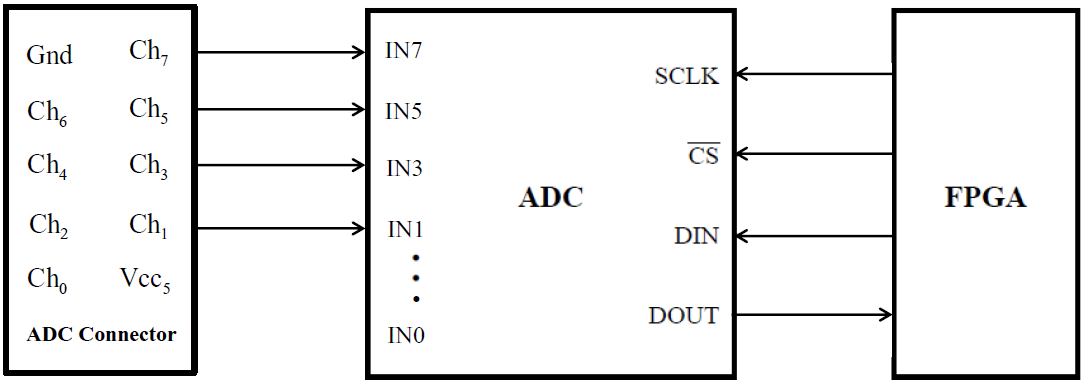
\includegraphics[scale = 0.47]{figures/signal_diagram.png}
\end{center}
\caption{Signals to and from the ADC on the \textbf{DE10-Standard}, \textbf{DE10-Nano}, \textbf{DE1-SoC}, and \textbf{DE0-Nano-SoC}}
\label{fig:signal}
\end{figure}

\begin{figure} [H]
\begin{center}
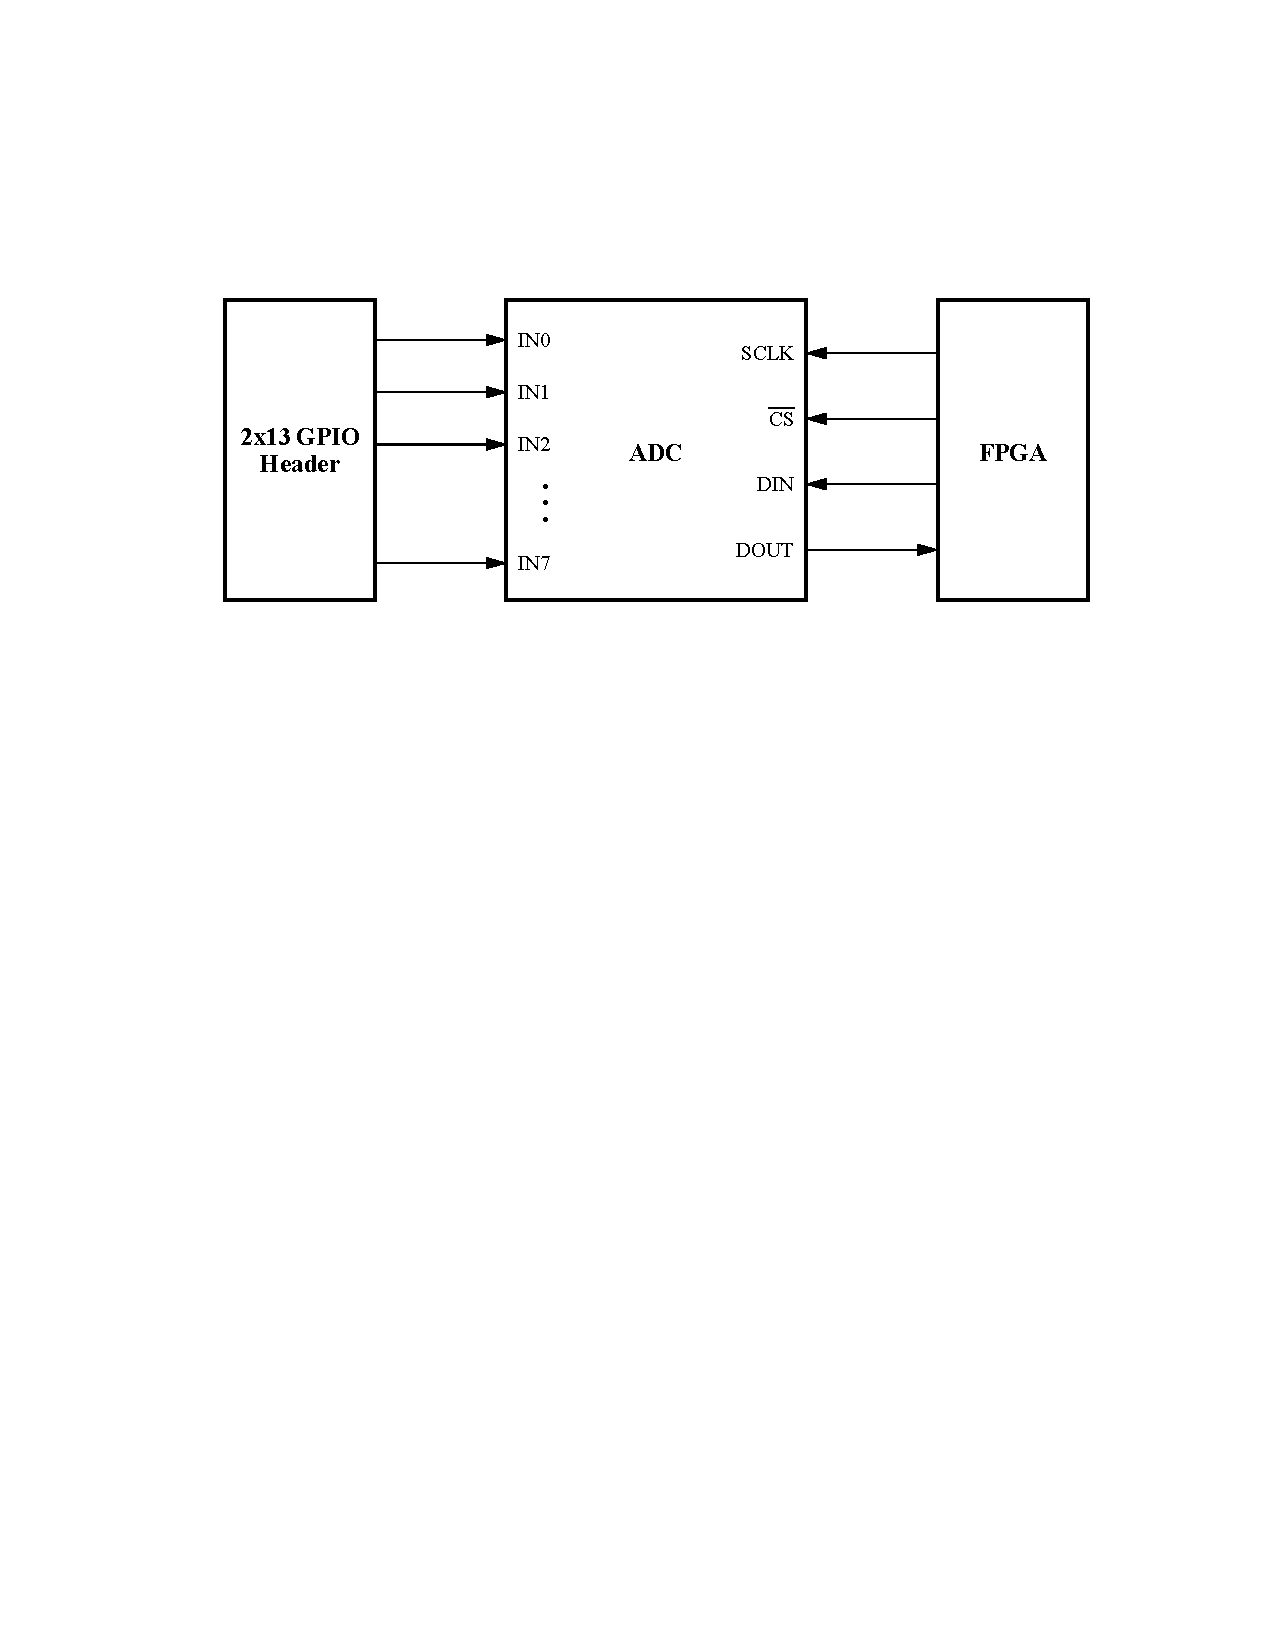
\includegraphics[scale = 0.9]{figures/signal_diagram_de0nano.pdf}
\end{center}
\caption{Signals to and from the ADC on the {\bf DE0-Nano} }
\label{fig:signal2}
\end{figure}

\begin{figure} [H]
\begin{center}
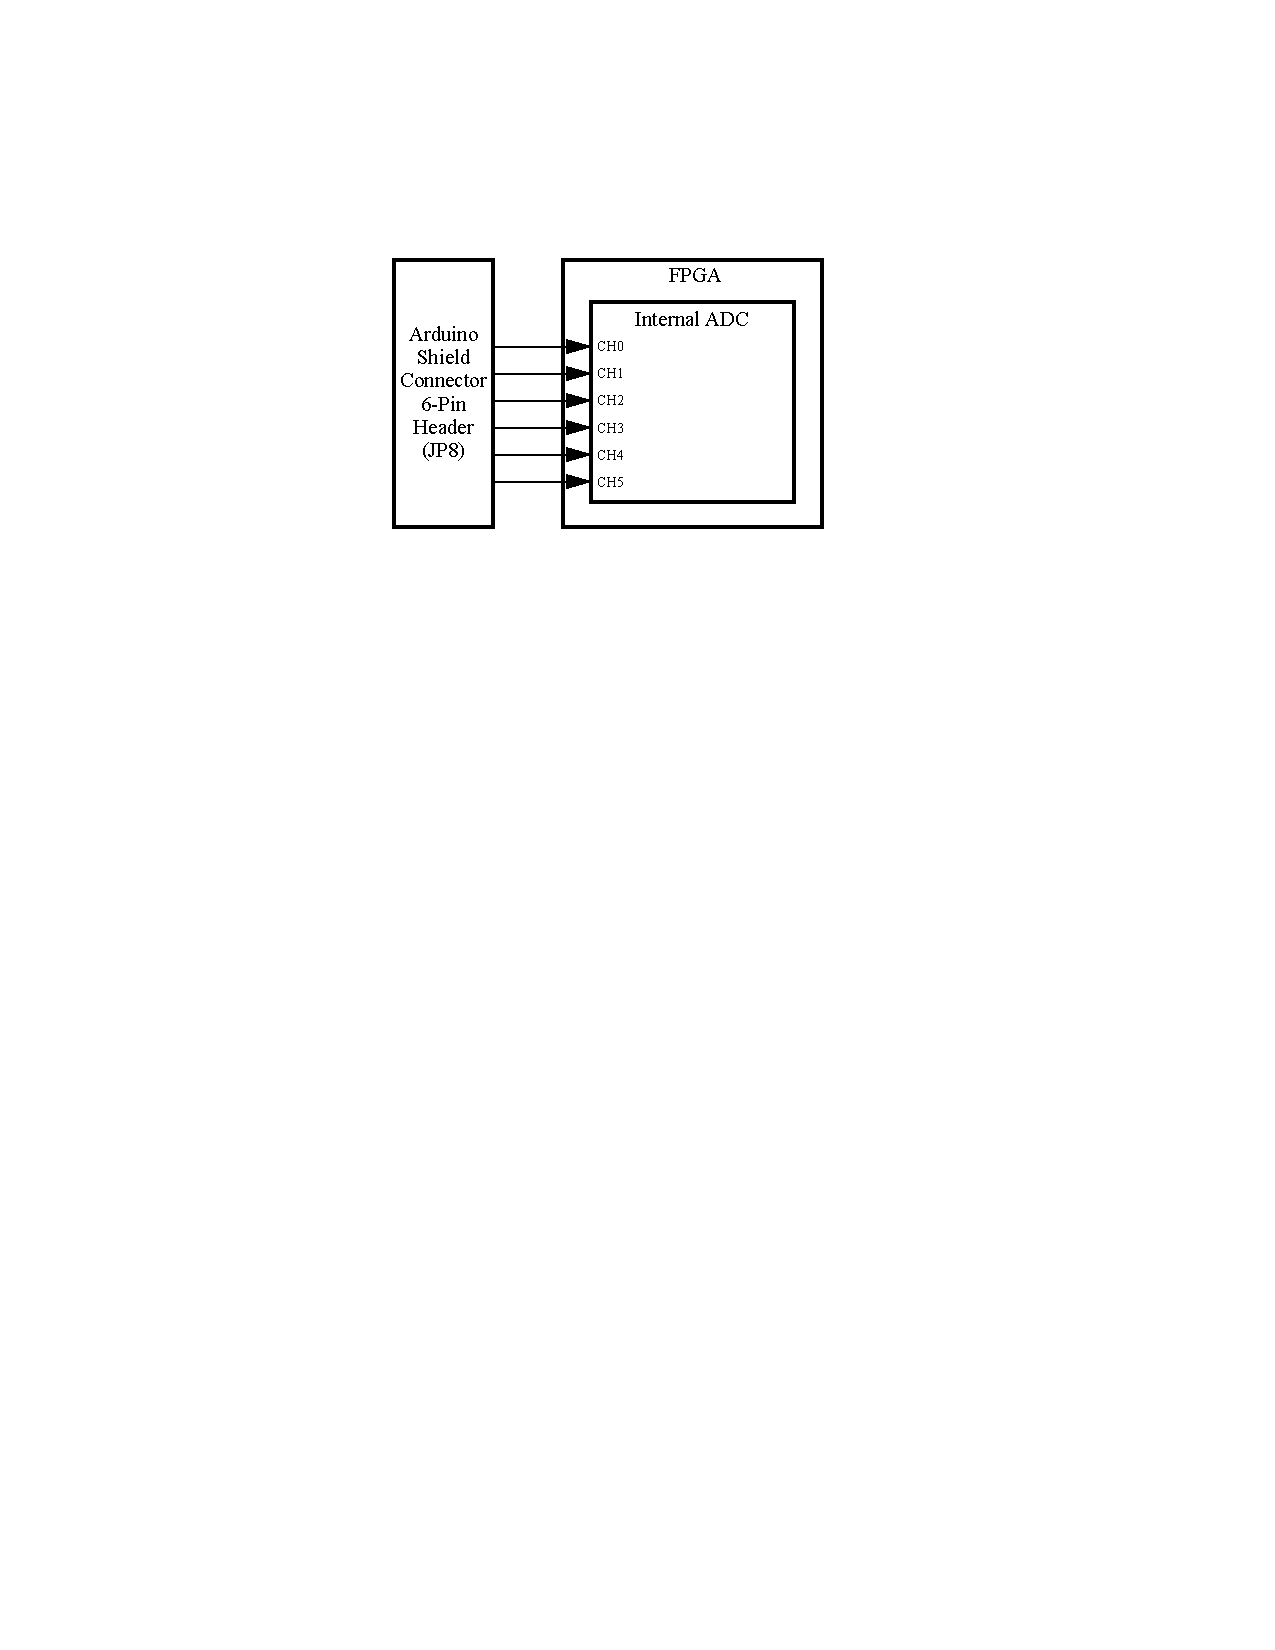
\includegraphics[scale = 1]{figures/signal_diagram_max10.pdf}
\end{center}
\caption{Signals to and from the ADC on the {\bf DE10-Lite} }
\label{fig:signal3}
\end{figure}

The ADC receives analog signals via its input pins (each corresponding to a channel). When performing a conversion, the ADC reads the signal on one of
these input channels and converts it to a digital output. On the DE10-Standard, DE10-Nano, DE0-Nano-SoC and DE1-SoC boards, these eight pins are connected to the dedicated 10-pin ADC header. 
On the DE0-Nano board, these eight pins are connected to the 2x13 GPIO header on the underside of the
board. On the DE10-Lite board, the six input pins are connected to the 6-Pin header of the Arduino* Shield Connectors. 

For all boards except the DE10-Lite (whose ADC is built into the FPGA), the ADC also has four wires connected to the FPGA. The wires are used to control the ADC and to allow communication between it and the FPGA. The {\it SCLK}  and $\overline{CS}$ signals are used to control the ADC, and are generated by circuitry in the FPGA. The {\it SCLK} signal serves as a device clock for the ADC, while the $\overline{CS}$ signal serves as an active-low chip select for the ADC chip. The {\it DIN} and {\it DOUT} wires are used for transferring addresses and data between the two chips. The FPGA uses the {\it DIN} connection, which is mapped to the {\it ADC\_SADDR} pin on the FPGA, to provide the address of the next channel requested for conversion. The address is 3 bits in length, and is sent to the ADC serially at a rate of 1 bit per {\it SCLK} cycle. The {\it DOUT} connection is mapped to the {\it ADC\_SDAT} pin on the FPGA, and is used by the ADC to send the digital value of the converted signal to the FPGA. This value is 12 bits long, and is sent to the FPGA in a serial manner at a rate of 1 bit per {\it SCLK} cycle.

\subsection{Timing and Signal Requirements}
Each boards ADC controller operates on a 16-cycle operational frame, as shown in Figure~\ref{fig:tim_req}. The user is required to provide the \textit{SCLK}, $\overline{CS}$, and \textit{DIN} signals to the ADC, and to capture the \textit{DOUT} signal as it is transmitted.

\begin{figure} [h]
\begin{center}
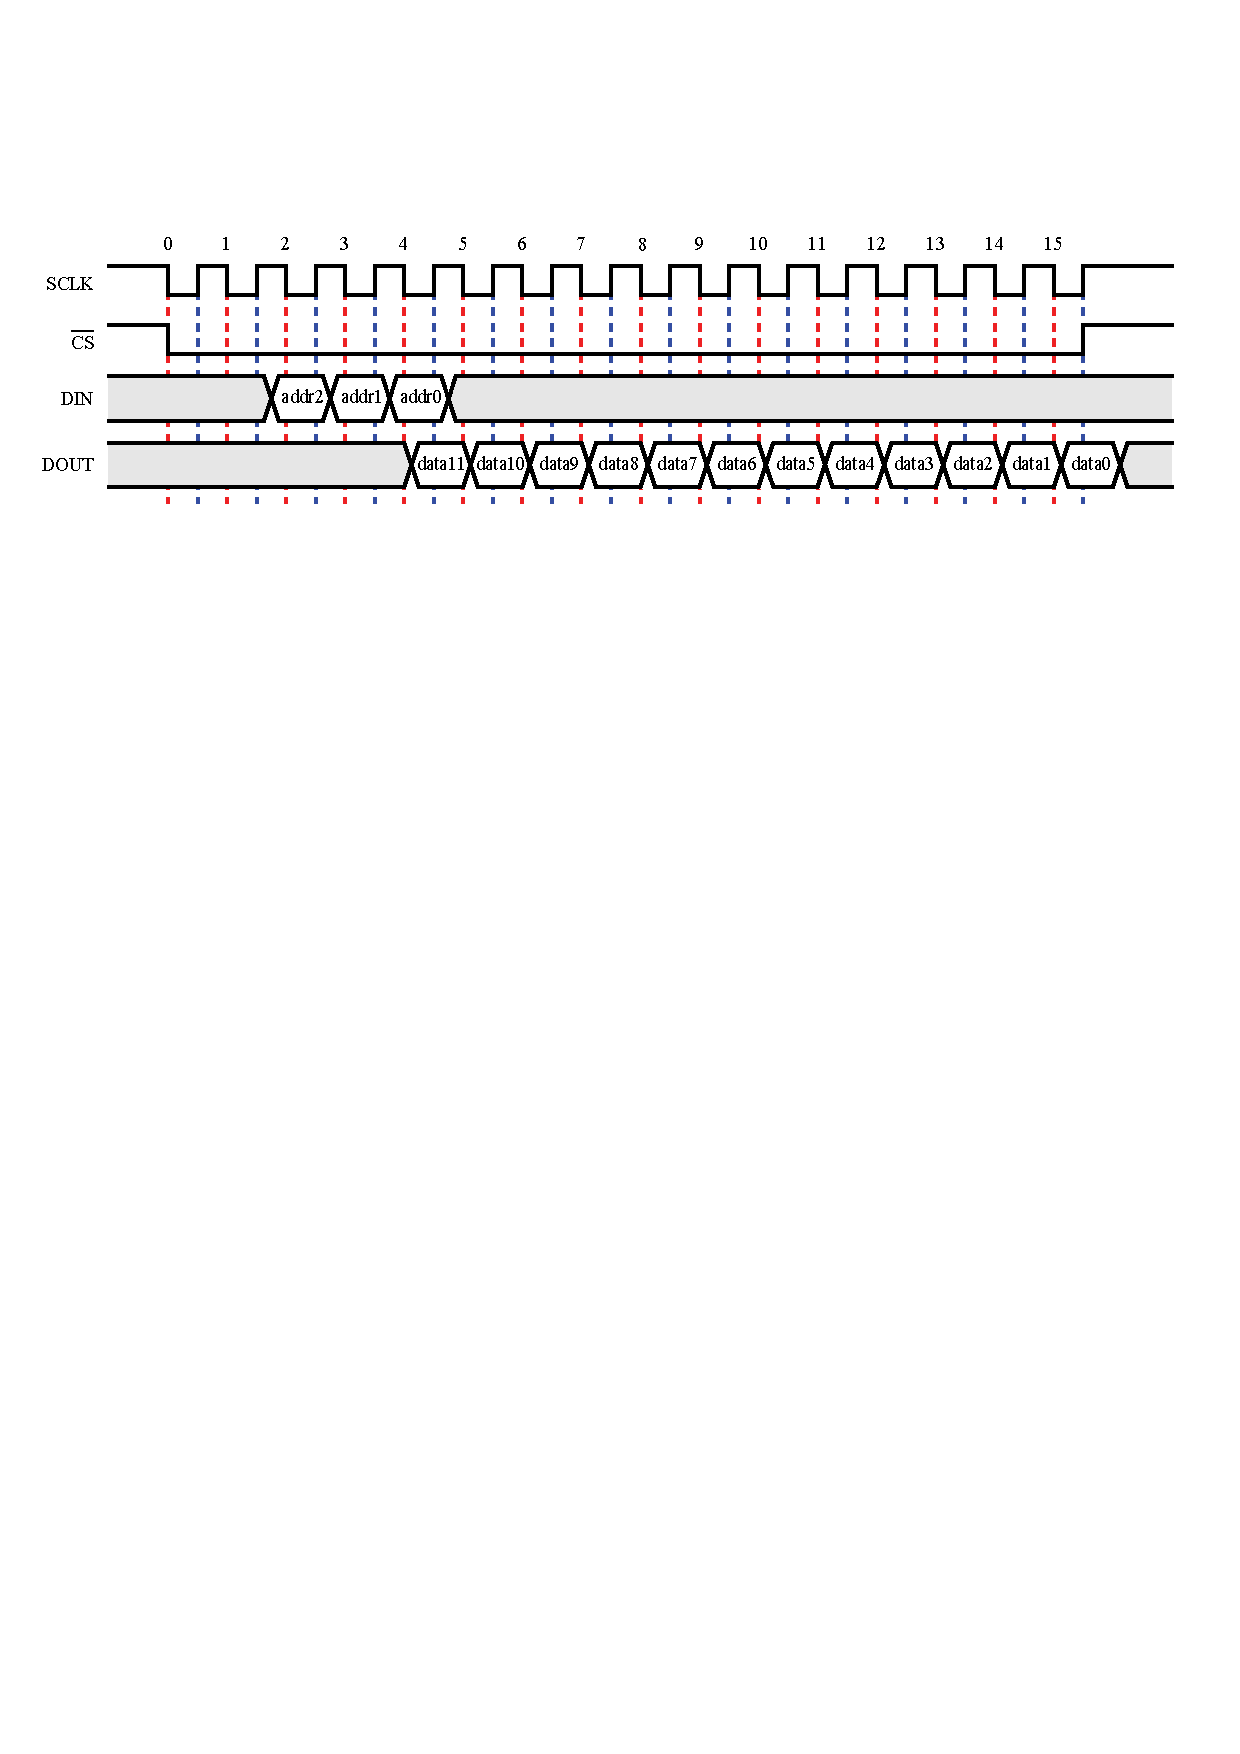
\includegraphics[scale=0.9]{figures/tim_req.pdf}
\end{center}
\caption{Timing requirements for the ADC}
\label{fig:tim_req}
\end{figure}

The \textit{DOUT} signal provides the 12-bit converted value of the selected channel. On power-up, \mbox{channel 0} is selected by default, while subsequent reads will use the address provided in the previous operational frame. The data bits are transmitted in descending order, such that the highest-order bit is delivered first. It is captured by the user on the rising edge of \textit{SCLK}.\\
\\
The \textit{DIN} signal is used to select the channel to be converted in the following frame. It is delivered in descending order, and is captured by the ADC on the positive edges of \textit{SCLK}. In order to avoid potential race conditions, the user should generate \textit{DIN} on the negative edges of \textit{SCLK}.\\
\\
$\overline{CS}$ should be lowered on the first falling edge of \textit{SCLK}, and raised on the last rising edge of an operational frame. 
See Table~\ref{tab:adc_info} for the timing requirements for each board.

\subsection{Analog Circuit Requirements}
All analog inputs are referenced against a {\sf Vdd} signal hardwired to the ADC. Therefore, to avoid damaging the boards, any voltages provided to the ADC
should not exceed this maximum voltage pins should not exceed the maximum voltages listed in 
Table~\ref{tab:adc_info}. If the analog circuitry is powered by a supply voltage greater than the maximum voltage, voltage dividers should be used to limit the
maximum output voltage to the maximum. Example analog circuits for measuring a variety of stimuli are shown in Figure~\ref{fig:analog_examples}. The resistance 
values given are approximate; all analog signals should be measured before being connected to the ADC.

\begin{figure} [H]
\begin {center}
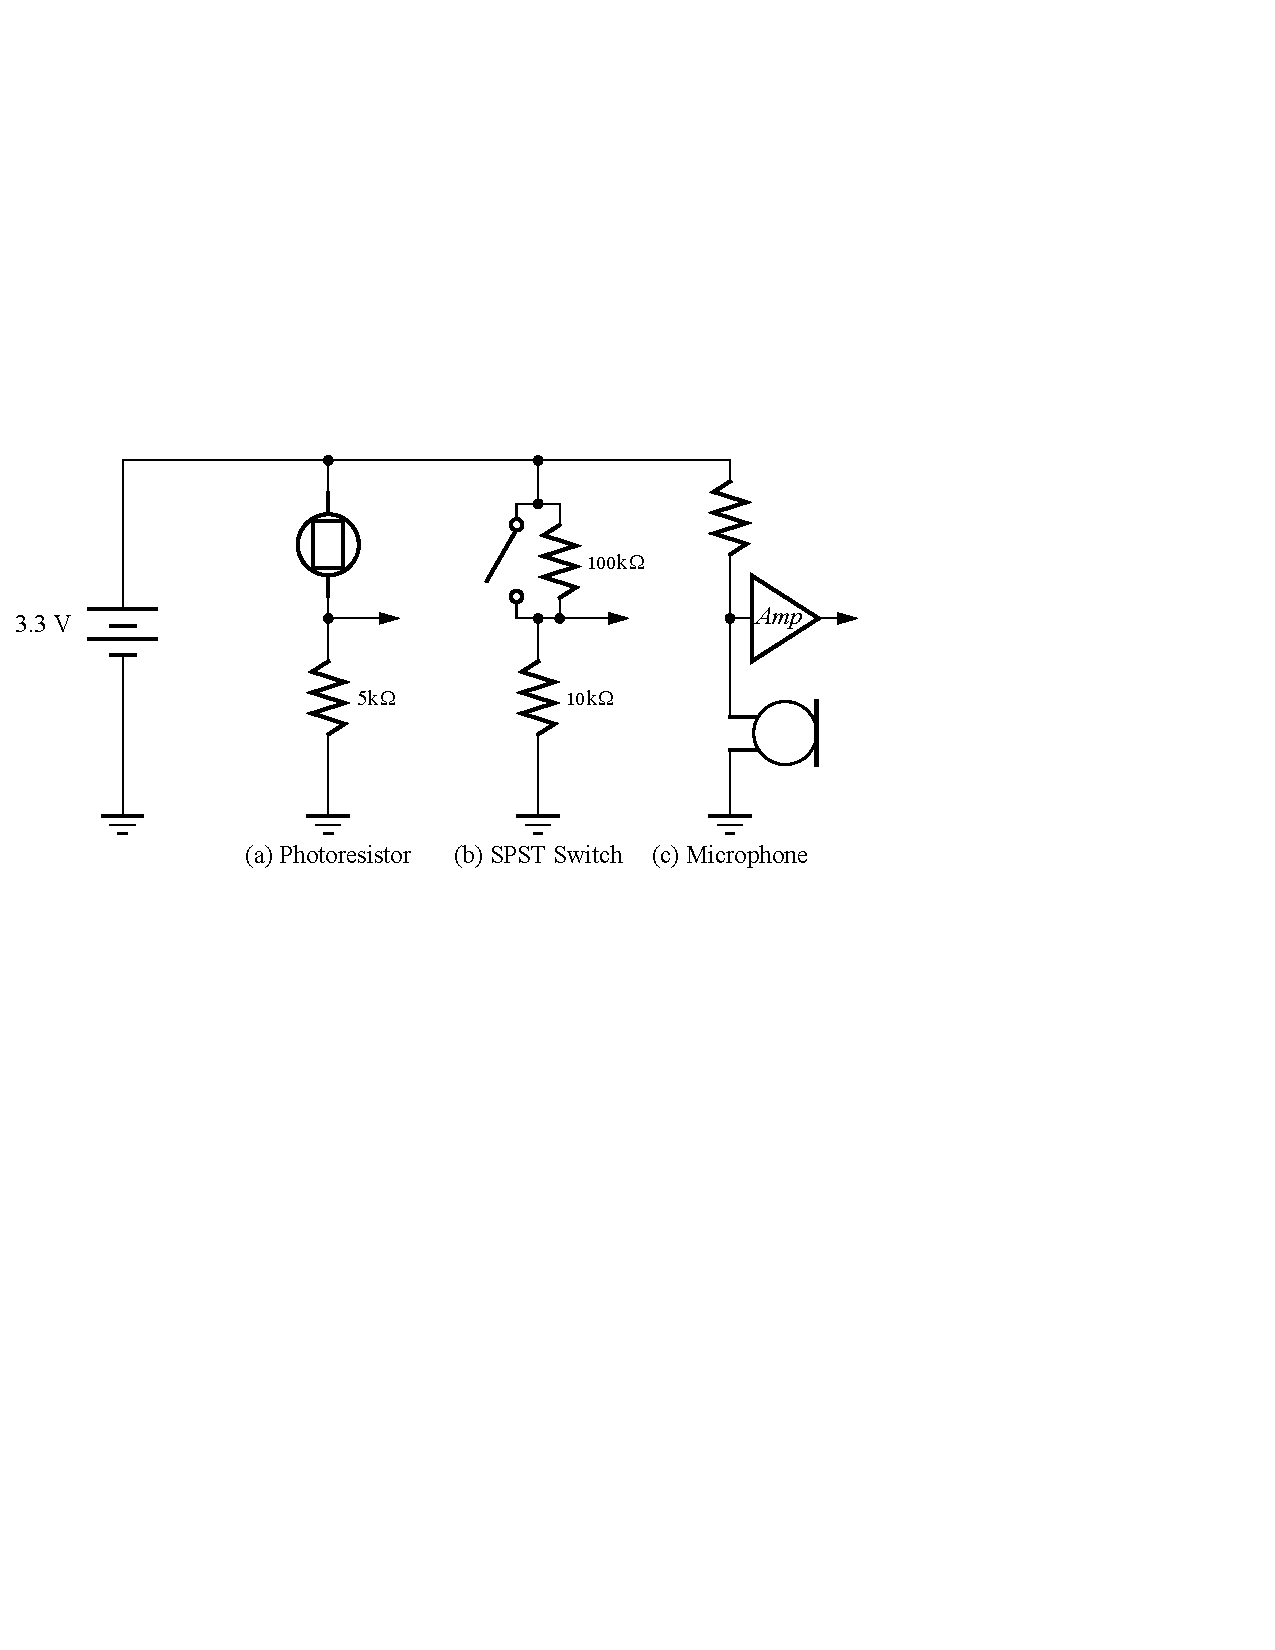
\includegraphics[scale=0.80]{figures/analog_examples.pdf}
\end{center}
\caption{Examples of analog circuits using a variety of sensors.}
\label{fig:analog_examples}
\end{figure}

Figure~\ref{fig:analog_examples}a includes a photoresistor. A photoresistor can be used to detect sources of light by changing resistance based upon the amount of light that strikes its surface. In this configuration, a high output voltage represents a bright signal, and low output represents a dark one. This can be reversed by switching the Vdd and GND connections.\\
\\
Figure~\ref{fig:analog_examples}b shows the usage of a simple switch. The output voltage is low when the switch is open, and high when the switch is closed. As with the photoresistor, this can be changed by swapping the Vdd and GND connections.\\
\\
Figure~\ref{fig:analog_examples}c utilizes a microphone. Since many basic microphones do not have a large enough signal amplitude to be detected by the ADC, the output may require amplification. The resistor should be matched to the impedance of the microphone.\\
\\
When connecting analog circuits to the ADC, it it essential to connect the ground potential of the circuit to the GND pin. This creates a common reference point 
for both the circuit and the board, so that voltages can be compared accurately. You can find and use a GND pin on your board by consulting the board's User Manual.
For example, you could use pin 10 of the 2x5 J15 ADC Controller header on the DE0-Nano-SoC and DE1-
SoC boards, or pin 26 of the 2x13 GPIO header on the DE0-Nano board. Figures~\ref{fig:analog_gpio} and ~\ref{fig:analog_gpio2} illustrate how an analog circuit 
should be connected to the board.
%\vfill
\begin {figure} [h]
\begin {center}
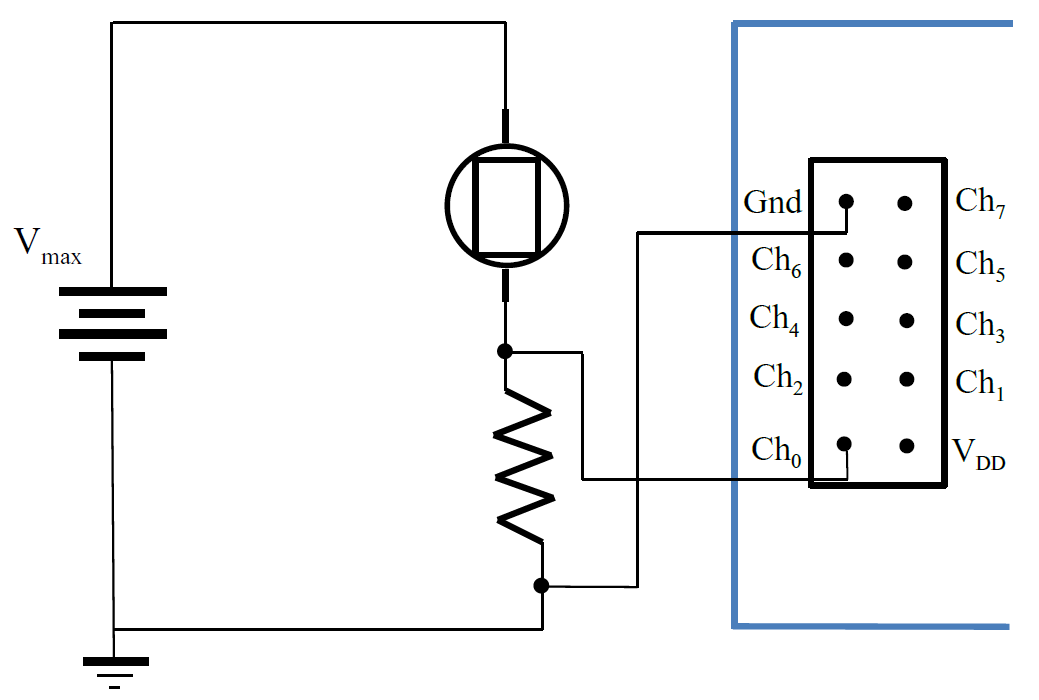
\includegraphics[scale=0.45] {figures/analog_gpio.png}
\end{center}
\caption {An analog circuit connected to the 2x5 ADC header on the {\bf DE10-Standard, DE10-Nano, DE0-Nano-SoC or DE1-SoC}.} 
\label{fig:analog_gpio}
\end {figure}

\begin {figure} [h]
\begin {center}
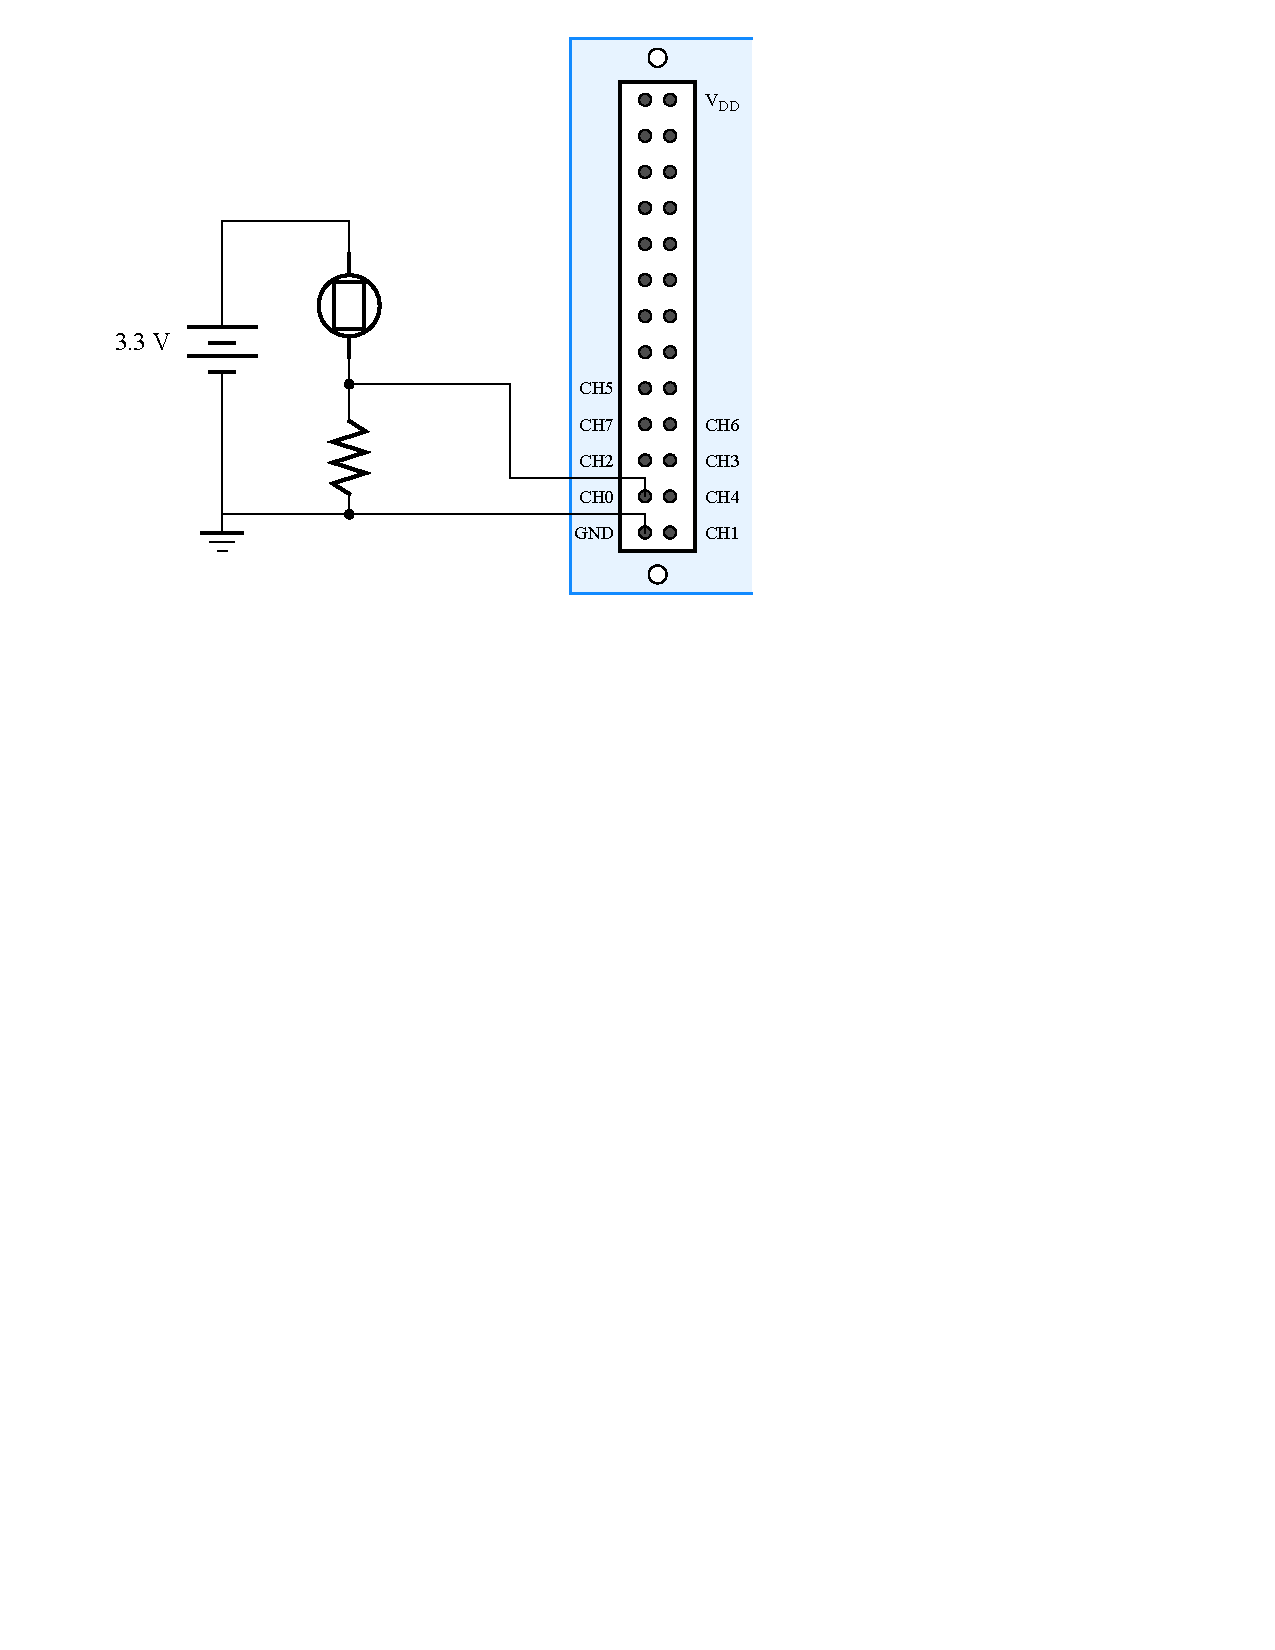
\includegraphics[scale=0.8] {figures/analog_gpio.pdf}
\end{center}
\caption {An analog circuit connected to the 2x13 GPIO header, shown from the underside of the {\bf DE0-Nano board}.}
\begin{center}The 2x13 GPIO should be on the right edge of the board.\end{center} 
\label{fig:analog_gpio2}
\end {figure}

\FloatBarrier
\section{The ADC Controller for DE-series Boards} 
The \textit{ADC Controller for DE-series Boards} IP Core manages and controls the signals between the ADC and FPGA, and provides the user with the converted values. The core is usable in both hardware-only and software-controlled versions. It reads each of the input channels of the ADC in ascending order once per update cycle, storing the acquired values locally. Once the update cycle is complete, the new values are available for access. It also provides a number of customizations to the user to control its operation.

The ADC controller core defines the number of channels in use as a parameter, {\it NUM\_CH}, which is set by the user when the core is instantiated. Since the core operates by sampling all used channels in series, reducing the number of used channels will reduce the total amount of time required to refresh the values.

The core also allows specification of the {\it SCLK} frequency. The user can enter a desired value in the allowed range (See Table~\ref{tab:adc_info}). 
Exact matching of the desired {\it SCLK} value is not guaranteed, as {\it SCLK} is derived as an integer factor of the system clock. Typically, the mismatch will be less than a 5\% difference between the desired and implemented value.

\subsection{Implementing the ADC Controller with the Platform Designer Tool}
\subsubsection{The Software-Controlled ADC Core}
For complex systems where a processor and software control is desired, the ADC controller can be included as a Platform Designer component compatible with a Nios\textsuperscript{\textregistered} II or ARM* processor. For information on designing systems in Platform Designer that include Nios II and/or ARM, refer to the {\it Introduction to the Intel Platform Designer Integration Tool} and {\it Introduction to the Intel Nios II Soft Processor} or {\it Introduction to the ARM A9 Processor} tutorials. 

The ADC Controller provides the processor with eight memory-mapped registers for reading and two registers for writing, as detailed in Table~\hyperref[tab:regfiles]{1}. The Controller is operated by reading from and writing to these registers.

\begin{table}[h]

    \centering
    \begin{tabular}{|c|c|c|p{7cm}|}
        \hline
        \multicolumn{4}{|l|}{\textit{\textbf{Table 2. DE-Series ADC Controller register map}}}
        \\\hline
            \textbf{Offset in bytes}
            & \textbf{Register name}
            & \textbf{Read/Write}
            & \textbf{Purpose}
        \\\hline
        \multirow{2}{*}{0} 
            & \texttt {CH\_0} & R & Converted value of channel 0
        \\\cline{2-4}
            & \texttt {Update} & W & Update the converted values
        \\\hline
        \multirow{2}{*}{4} 
            & \texttt {CH\_1} & R & Converted value of channel 1
        \\\cline{2-4}
            & \texttt {Auto-Update} & W & Enables or disables auto-updating
%        \\\hline
%        \multirow{2}{*}{8} 
%            & \texttt {CH\_2} & R & Converted value of channel 2.
%        \\\cline{2-4}
%            & \texttt {SCLK Counter} & W & Set the SCLK frequency.
        \\\hline
            8
            & \texttt{CH\_2}
            & R
            & Converted value of channel 2
        \\\hline
            12
            & \texttt{CH\_3}
            & R
            & Converted value of channel 3
        \\\hline
            16
            & \texttt{CH\_4}
            & R
            & Converted value of channel 4
        \\\hline
            20
            &\texttt{CH\_5}
            & R
            & Converted value of channel 5
        \\\hline
            24
            & \texttt{CH\_6}
            & R
            & Converted value of channel 6
        \\\hline
            28
            & \texttt{CH\_7}
            & R
            & Converted value of channel 7
        \\\hline
    \end{tabular}
    \label{tab:regfiles}
\end{table}

For reading, each of the eight registers corresponds to one of the eight input channels to the ADC. After the ADC converts the desired number of channels, the
converted values will be available in these registers. If a channel is not in use, its corresponding register will contain zeroes. In each channel register,
the low 12 bits (bits 11 to 0) are the value of the analog signal. Bit 15 in each register is a {\it refresh} bit, which is used in Auto-update mode. The 
bit is set to 1 when a corresponding channel is refreshed, and set to 0 when read. The remaining bits (31 to 16 and 14 to 12) are unused.

The \textit{Update} register is used to initiate a conversion operation. Performing a write to this register will update all channels in use, with the new values becoming available once the entire conversion process has finished. If reads to the channel registers are attempted while a conversion is taking place, then the {\it wait\_request} signal will be raised, causing the processor to stall until the update has finished.

The \textit{Auto-Update} register is initially loaded with a zero value. The auto-update allows the system to automatically begin a second update cycle after the first finishes. As result, channel values can be accessed during an update cycle, and it is user's responsibility to ensure the values used are up-to-date. Writing a `1' to this register enables auto-update, while writing a `0' disables it.

\subsubsection{Using the ADC Controller Core}
To demonstrate the use of the ADC Controller, we will implement a system using the Platform Designer tool for the DE0-Nano-SoC board. The system will be controlled by a processor and software, and the converted values from the ADC will be displayed on the board's LEDs. Although we will use the DE0-Nano-SoC for demonstration purposes, similar steps can be used for other DE-series boards.

To make a new system with the ADC Controller, create a new project in Quartus Prime named {\it adc\_demo}. The top-level module should also be {\it adc\_demo}. Specify the device as the Cyclone\textsuperscript{\textregistered} VE chip {\bf 5CSEMA4U23C6}, and complete the project creation. Then, open the Platform Designer tool.

The system will have four main components: the ADC Controller, a Nios II processor, on-chip memory, and LEDs to display the read values. The block diagram of the system is shown in Figure~\ref{fig:sys_diagram}.
\begin {figure} [H]
\begin {center}
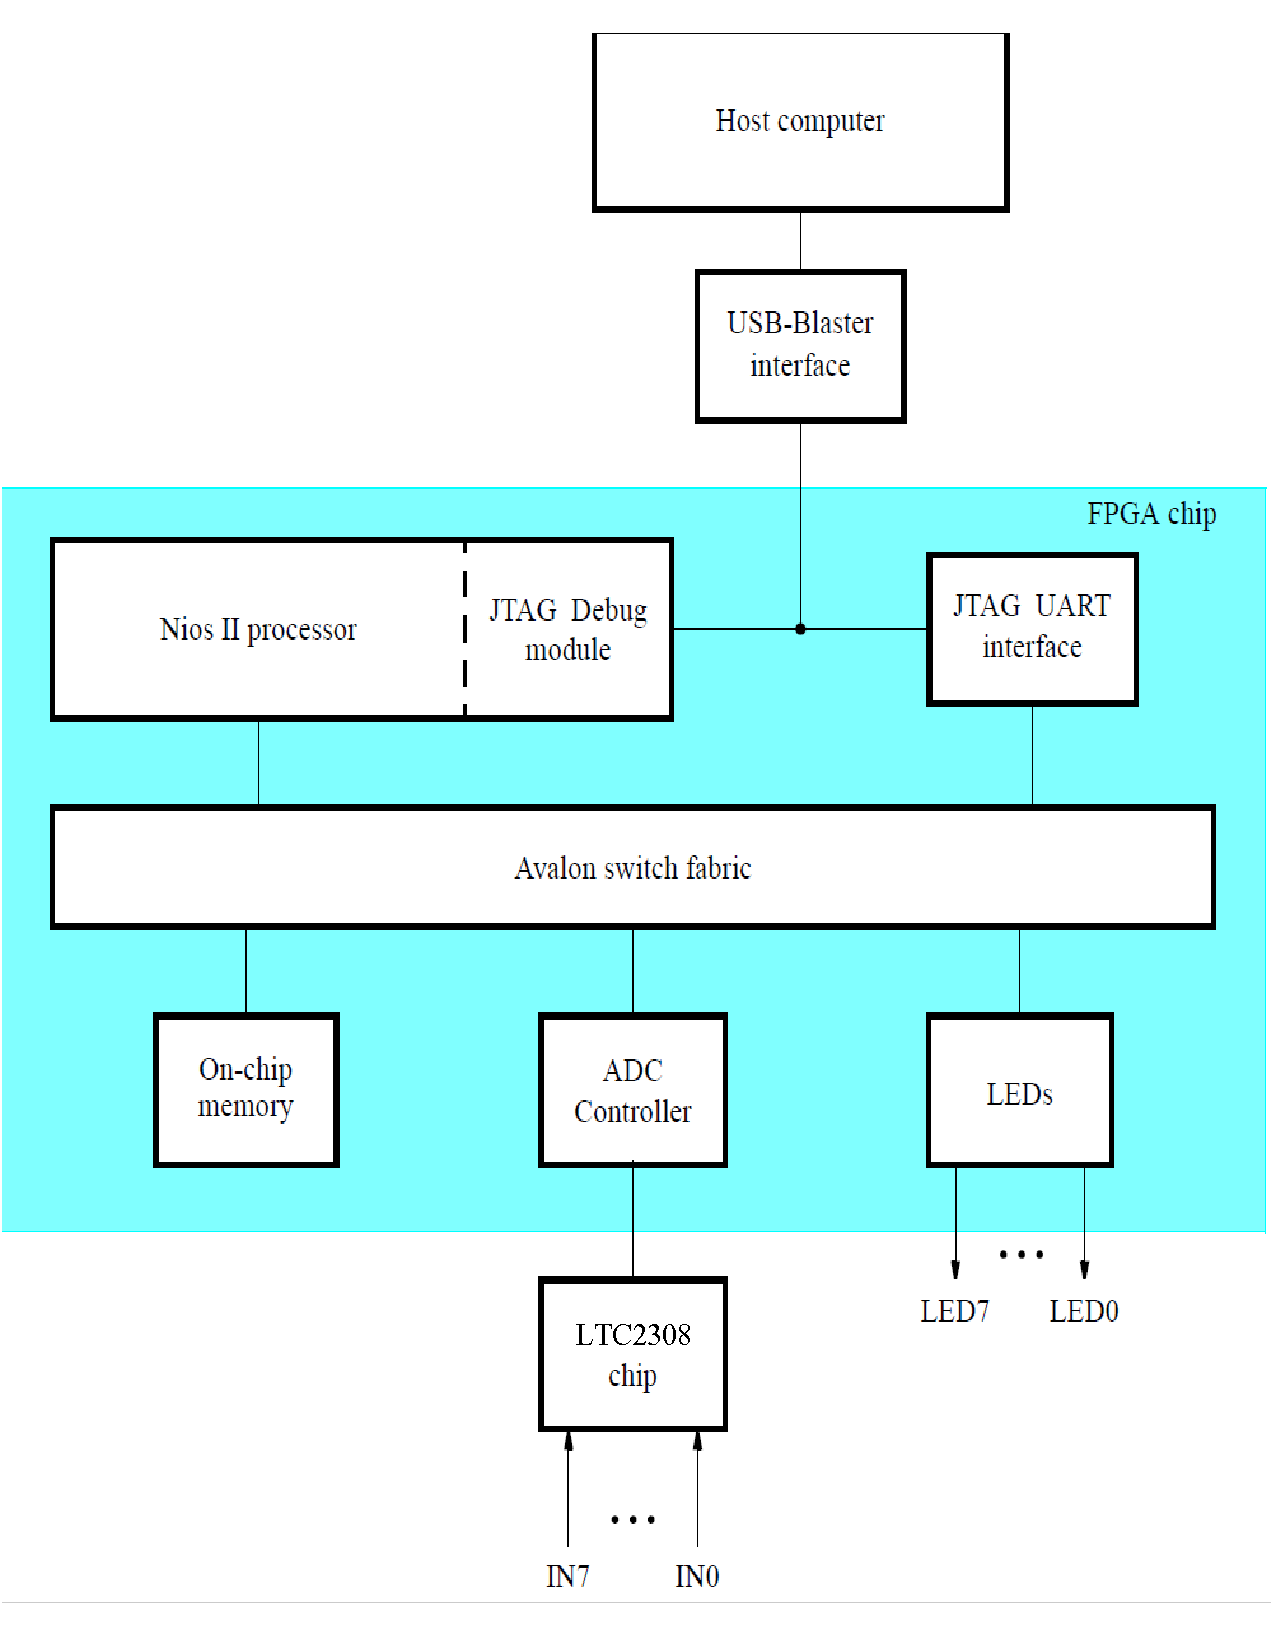
\includegraphics [scale = 0.60]{figures/system_diagram.pdf}
\end {center}
\caption{A simple Nios II system with the ADC Controller.}
\label{fig:sys_diagram}
\end {figure}

The system will use a 100 MHz system clock instead of CLOCK\_50. First remove, the default clock source that is included in the new Platform Designer project. Next, from {\sf University Program}, select the {\sf System and SDRAM Clocks for DE-series Boards} from the {\sf Clock} list. Change the Desired System clock to ``100.0'' MHz and the DE-Series Board to {\sf DE0-Nano-SoC}, then select {\sf Finish}. Export the Clock Input as {\sf clk} and the Reset Input as {\sf reset}. Use {\sf sys\_clk} as the system clock and {\sf reset\_source} as the system reset.

From the {\sf Processors and Peripherals}, select the {\sf Nios II Processor} from the {\sf Embedded Processors} list. Select {\sf Nios II/e} as the processor type and add the processor to the system. Rename this module to {\it cpu}, and connect it to the clock and reset signals.

Next add the on-chip memory by selecting {\sf On-Chip Memory (RAM or ROM) Intel FPGA IP} from the {\sf Basic Functions > On Chip Memory} component list. Specify ``8192'' as the total memory size and select {\sf Finish} to add it to the system. Connect the clock and reset signals to the memory, and connect the memory to the data\_master and instruction\_master sources of the Nios II processor. Rename the memory to {\it onchip\_mem}. Edit the Nios II processor to specify {\it onchip\_mem} as the reset and exception vector memories.

Use a {\sf PIO (Parallel I/O)} component to connect the system to the LEDs. Select {\sf Processors and Peripherals > Peripherals} and choose  the {\sf PIO (Parallel I/O)} component. Specify a width of 8, and select Output as the direction. Rename the component to {\it LEDs}. Connect it to the clock and reset sources, the Nios II data\_master, and export the conduit as {\it leds}.\\
\begin {figure} [H]
\begin {center}
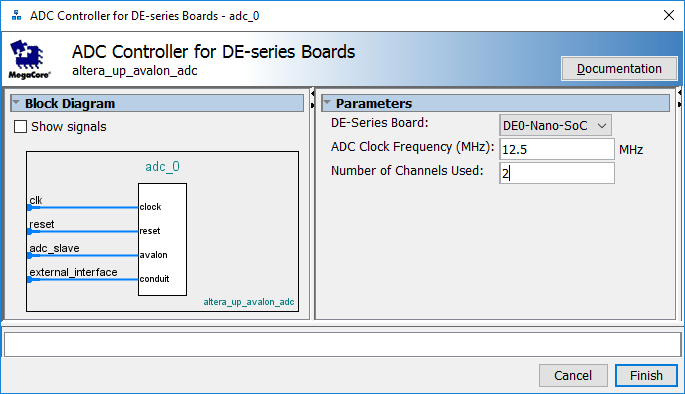
\includegraphics [scale = 0.7] {figures/adc_comp.png}
\end {center}
\caption {The ADC Controller component window.}
\label {fig:adc_comp}
\end {figure}

Lastly, include the ADC controller in the system by selecting {\sf University Program > Generic IO > ADC Controller for DE-Series Boards} from the component list. Select the DE0-Nano-SoC board and specify ``2'' as the number of channels used, then select {\sf Finish} to add it to the system. After adding the ADC controller to your system, rename the component to {\it ADC}. Connect the {\it clk}, {\it reset} and {\it adc\_slave} signals to the clock source, clock reset and data\_master sources, and export the {\it external\_interface} signal as {\it adc}. Note: the ADC controller for the DE-10 Lite board does not contain an external\_interface signal, as the connections are internal to the FPGA. \\
\\
Assign the component addresses by selecting {\sf System > Assign Base Addresses}. The system should match the one presented in Figure~\ref{fig:qsys_adc}. Take note of the addresses assigned to the LEDs and the ADC controller, as these will be needed later. Save the system as {\it nios\_system} and generate it using {\sf Generate > Generate HDL...}.


\begin {figure} [H]
\begin {center}
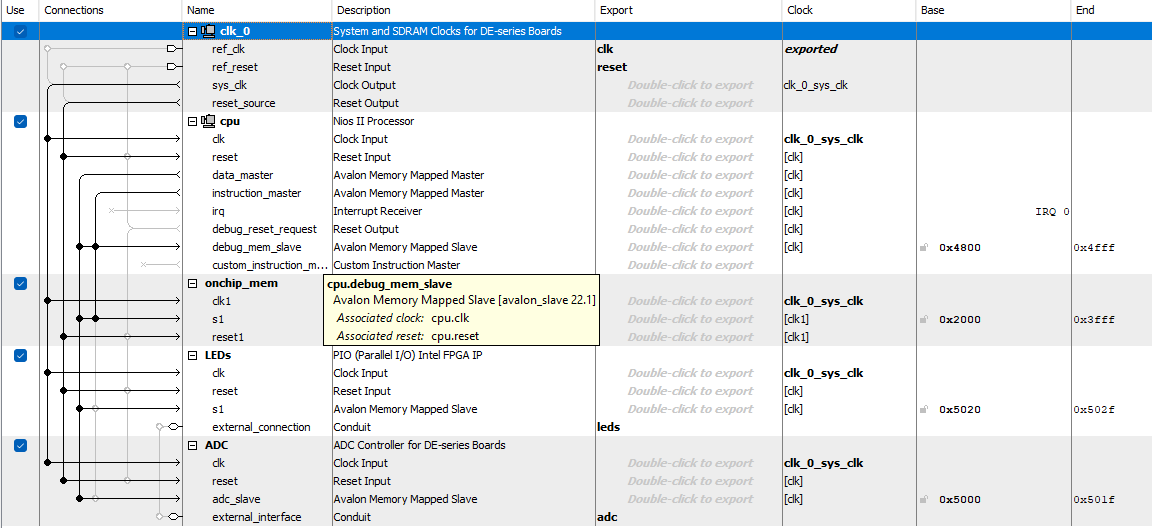
\includegraphics [scale = 0.7] {figures/qsys_adc.png}
\end{center}
\caption {The system in Platform Designer with the ADC Controller.}
\label {fig:qsys_adc}
\end{figure}

After generating the system, it is necessary to create a top-level module for the system. Create a new verilog file and copy the code from Figure~\ref{fig:top_level} into it, or use the one provided in the ``design files'' subdirectory. Save this file as {\it adc\_system.v}. Add the top level file just created and the {\it synthesis/nios\_system.qip} file to project file list. Import the DE0-Nano-SoC Pin Assignments file and compile the project.

\begin{figure}[H]
\lstinputlisting[language=Verilog, xleftmargin=3cm]{design_files/adc_demo.v}
\caption{Example top-level module for a project using the ADC Controller.}
\label{fig:top_level}
\end{figure}

To use the ADC in a C program, declare a {\bf volatile int *} for each peripheral, such as the ADC or LEDs. Assign this pointer the base address of the component as it was defined in Platform Designer. To read from or write to the component, use the dereference operator (*) to read or write values as appropriate. For peripherals with multiple registers, such as the ADC controller, treat the peripheral as an array of integer-sized values.\\
\\
Example C code for operating the ADC is shown in Figure~\ref{fig:c_code}, and is available for use in the ``design files'' subdirectory. This code uses the first two channels of the ADC, alternating between them every \mbox{500,000} reads. The highest 8 bits for the channel will be displayed on the LEDs.\\
\begin{figure}
\lstinputlisting[language=C, xleftmargin=1.5cm]{design_files/main.c}
\caption{C code to operate the ADC.}
\label{fig:c_code}
\end{figure}

Use the \productNameMed{} to download the system and C program to the FPGA chip. Users unfamiliar with the \productNameMed{} should consult the {\it \productNameMed{} Tutorial} for a detailed description of the program's features. To begin, create a new project using a custom system. Use the {\it .sopcinfo} generated by Platform Designer and the {\it .sof} file generated by Quartus to define the system. Next, choose {\sf C Program} as the program type, and include the relevant C file. Leave all other settings unchanged, complete project creation and compile the program. After compilation is finished, load the program and select {\sf Actions > Continue} to run it.

%\FloatBarrier
\clearpage
\newpage
\subsection{Using the ADC Controller with HAL}

Alternatively, it is possible to use a processor and the various peripherals without creating a custom system. In this case, it is advantageous to use the {\it Hardware Abstraction Layer} or HAL. The HAL allows the use of task-specific function calls for accessing the peripheral, instead of accessing the peripheral directly. Additional details on the HAL can be found in the {\it Using HAL Device Drivers with the \productNameMed{}} tutorial. The documentation for all University Program HAL devices can be found in the {\sf [Quartus Directory]/ip/University\_Program} directory.\\
\\
The HAL Driver for the ADC offers five functions for accessing and controlling the ADC. To use these functions, the program must include the statement:\\
\qquad\texttt{\#include "altera\_up\_avalon\_adc.h"}\\
\\
The first step when using the ADC with HAL is to create a device pointer to the ADC. HAL device drivers feature a different variable type for each device; for the ADC controller, the type ``{\it alt\_up\_adc\_dev}'' is used. After creating the pointer, the value is assigned using the {\it alt\_up\_adc\_open\_dev (...)} function. This function takes in the name of the device and locates it within the system, and returns a pointer to the adc controller. If the default system is used,  the string {\it ``/dev/ADC''} should be used; otherwise, replace ADC with the name of the component as defined in the Platform Designer system. The result of this function should be assigned to the device pointer created for the ADC.\\
\\
Once initialized, the other four functions can be used as desired. Definition prototypes and detailed descriptions for the HAL functions are shown in Figure~\ref{fig:hal_func}. An alternative version of the C example presented above - now using the HAL - is shown in Figure~\ref{fig:hal_code}, and in the ``design files'' subdirectory.\\

Having completed the code, load the program into the FPGA using the \productNameMed{}. As in the previous section, a custom system can be used, though the use of HAL does allow the use of the {\it DE0-Nano-SoC Computer} instead. Additionally, instead of specifying the program type as {\sf C Program}, choose {\sf Program with Device Driver Support}. This option will include any relevant HAL drivers automatically during compilation, but the program will require significantly more memory. If the program is too large to fit in the on-chip memory, consider implementing an SDRAM module to provide additional memory for the system.\\
\\
Compile and load the system and program to test the device.

\begin{figure}[h]

\begin{flushleft} %%%\begin{singlespace}
\parbox{12.5cm}{
{\small \textsf{\textbf{alt\_up\_de0\_nano\_adc\_open\_dev}}} \\
\begin{tabular}[ht]{lp{11cm}}
	\textbf{Prototype:}
	&
	\texttt{alt\_up\_adc\_dev* alt\_up\_adc\_open\_dev( const char *name)} 
	\\
	\textbf{Include:}
	&
	{\tt <altera\_up\_avalon\_adc.h>}
	\\
	{\textbf{Parameters:}}
	&
	\texttt{{name}}
	 -- the ADC Controller name. For example, if the ADC controller name in Platform Designer is "ADC", then {\it name} should be "/dev/ADC" 
	\\
	\textbf{Returns:}
	& The corresponding device structure, or NULL if the device is not found.
	\\
	\textbf{Description:}
	& Open the ADC controller device specified by {\it name} .\\
\end{tabular}
\\
\\
\\
{\small \textsf{\textbf{alt\_up\_adc\_read}}} \\
\begin{tabular}[ht]{lp{11cm}}
	\textbf{Prototype:}
	&
	\texttt{unsigned int alt\_up\_adc\_read ( alt\_up\_adc\_dev *adc, unsigned channel)} 
	\\
	\textbf{Include:}
	&
	{\tt <altera\_up\_avalon\_adc.h>}
	\\
	{\textbf{Parameters:}}
	&
	\texttt{{adc}}
	 -- struct for the ADC controller device . 
	\\
	&
	\texttt{{channel}}
	 -- the channel to be read, from 0 to 7.
	 \\
	\textbf{Returns:}
	& data -- The converted value from the desired channel.
	\\
	\textbf{Description:}
	& Read from a channel of the ADC.\\
\end{tabular}
\\
\\
\\
{\small \textsf{\textbf{alt\_up\_\_adc\_update}}} \\
\begin{tabular}[ht]{lp{11cm}}
	\textbf{Prototype:}
	&
	\texttt{void alt\_up\_\_adc\_update( alt\_up\_adc\_dev *adc)} 
	\\
	\textbf{Include:}
	&
	{\tt <altera\_up\_avalon\_adc.h>}
	\\
	{\textbf{Parameters:}}
	&
	\texttt{{adc}}
	 -- struct for the ADC controller device . 
	\\
	\textbf{Description:}
	& Trigger the controller to convert all channels and store the values.\\
\end{tabular}
\\
\\
\\
{\small \textsf{\textbf{alt\_up\_adc\_auto\_enable}}} \\
\begin{tabular}[ht]{lp{11cm}}
	\textbf{Prototype:}
	&
	\texttt{void alt\_up\_adc\_auto\_enable( alt\_up\_adc\_dev *adc)} 
	\\
	\textbf{Include:}
	&
	{\tt <altera\_up\_avalon\_adc.h>}
	\\
	{\textbf{Parameters:}}
	&
	\texttt{{adc}}
	 -- struct for the ADC controller device . 
	\\
	\textbf{Description:}
	& Enable automatic converting of channels.\\
\end{tabular}
\\
\\
\\
{\small \textsf{\textbf{alt\_up\_adc\_auto\_disable}}} \\
\begin{tabular}[ht]{lp{11cm}}
	\textbf{Prototype:}
	&
	\texttt{void alt\_up\_adc\_auto\_disable( alt\_up\_adc\_dev *adc)} 
	\\
	\textbf{Include:}
	&
	{\tt <altera\_up\_avalon\_adc.h>}
	\\
	{\textbf{Parameters:}}
	&
	\texttt{{adc}}
	 -- struct for the ADC controller device . 
	\\
	\textbf{Description:}
	& Disable automatic converting of channels.\\
\end{tabular}
 } %%%\end{singlespace}
	\caption{HAL functions for the ADC controller. }%(Part \it{a})}
	\label{fig:hal_func}
\end{flushleft}
\end{figure} 
%\FloatBarrier
%\begin{center} %%%\begin{singlespace}
%\parbox{12.5cm}{
%{\small \textsf{\textbf{alt\_up\_de0\_nano\_adc\_set\_sclk\_counter}}} \\
%\begin{tabular}[ht]{lp{11cm}}
%	\textbf{Prototype:}
%	&
%	\texttt{void alt\_up\_de0\_nano\_adc\_set\_sclk\_counter( alt\_up\_de0\_nano\_adc\_dev *adc, unsigned sclk\_count)} 
%	\\
%	\textbf{Include:}
%	&
%	{\tt <altera\_up\_avalon\_de0\_nano\_adc.h>}
%	\\
%	{\textbf{Parameters:}}
%	&
%	\texttt{{adc}}
%	 -- struct for the ADC controller device . 
%	\\
%	&
%	\texttt{{sclk\_count}}
%	 -- the new value for the SCLK counter.
%	\\
%	\textbf{Description:}
%	& Set the frequency of SCLK by changing the ratio of system clock cycles per SCLK cycle.\\
%\end{tabular}
%\\
%\\
%\\{\small \textsf{\textbf{alt\_up\_de0\_nano\_adc\_set\_sclk\_freq}}} \\
%\begin{tabular}[ht]{lp{11cm}}
%	\textbf{Prototype:}
%	&
%	\texttt{void alt\_up\_de0\_nano\_adc\_set\_sclk\_freq( alt\_up\_de0\_nano\_adc\_dev *adc, float sclk\_freq, float sysclk\_freq)} 
%	\\
%	\textbf{Include:}
%	&
%	{\tt <altera\_up\_avalon\_de0\_nano\_adc.h>}
%	\\
%	{\textbf{Parameters:}}
%	&
%	\texttt{{adc}}
%	 -- struct for the ADC controller device . 
%	\\
%	&
%	\texttt{{sclk\_freq}}
%	 -- the desired value for SCLK, in MHz.
%	\\
%	&
%	\texttt{{sysclk\_freq}}
%	 -- the system clock frequency in MHz. Typically 50MHz on DE0-Nano boards.
%	\\
%	\textbf{Description:}
%	& Set the frequency of SCLK. This function provids an alternate interface to the \texttt{alt\_up\_de0\_nano\_adc\_set\_sclk\_freq} function.\\
%\end{tabular}
%\\
%\\
%} %%%\end{singlespace}
%\\
%\begin{center}
%Figure~\ref{fig:hal_func}. HAL functions for the ADC controller. (Part \it{b}).
%\end{center}
%\vfill

\begin{figure}
\lstinputlisting[language=C, xleftmargin=2cm]{design_files/main_hal.c}
\caption{C code using HAL to operate the ADC.}
\label{fig:hal_code}
\end{figure}

\FloatBarrier
\subsection{Using the ADC Controller with IP Catalog}
To include the ADC controller in a hardware-based project, use the IP Catalog. Basic information on using the IP Catalog can be found in the {\it Using the Library of Parameterized Modules (LPM)} tutorial. The IP Catalog version of the controller allows access to between two and eight channels, with channel values updating automatically. 
\\

To instantiate the controller, open {\sf Tools > IP Catalog}. Select {\sf University Program > Generic IO > ADC Controller for DE-series boards}. The window in Figure~\ref{fig:ipcatalog1} will appear. Set the values to match the figure and press {\sf OK}. The window in Figure~\ref{fig:ipcatalog2} will appear. Set the parameters of the ADC controller to those listed in the figure and then press {\sf Generate HDL...} which will cause the window in Figure~\ref{fig:ipcatalog3} to appear. Press {\sf Generate} to generate the system. The window in Figure~\ref{fig:ipcatalog4} may appear, if it does press {\sf Close} after the system saves to continue the generation of HDL.

\begin {figure} [H]
\begin {center}
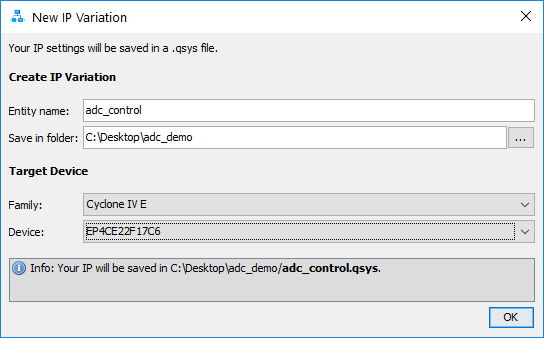
\includegraphics [scale = 0.6] {figures/ipcatalog1.png}
\end {center}
\caption {Creating a new IP variation of the ADC controller.}
\label {fig:ipcatalog1}
\end {figure}

\begin {figure} [H]
\begin {center}
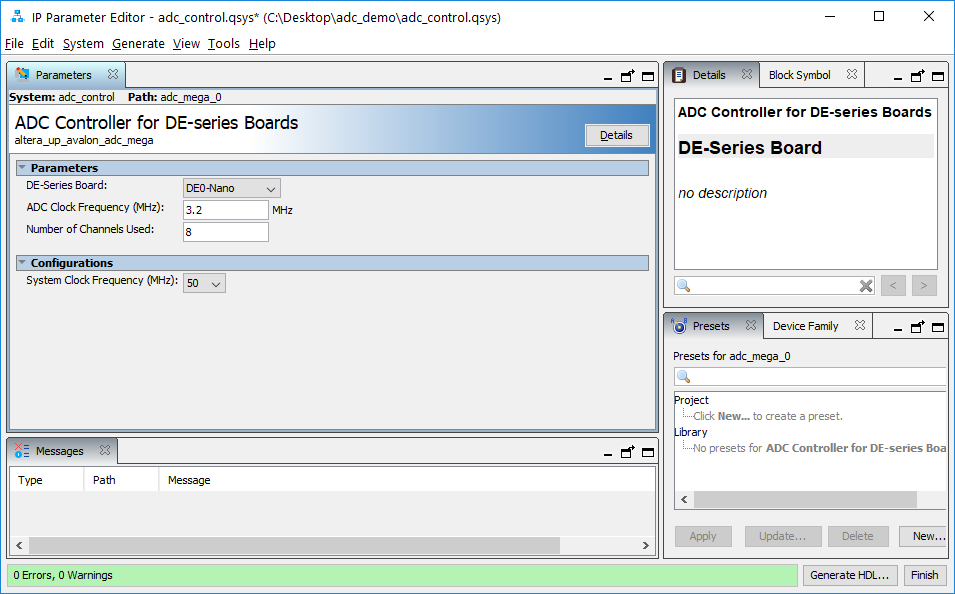
\includegraphics [scale = 0.6] {figures/ipcatalog2.png}
\end {center}
\caption {Configuring the ADC controller in the IP Catalog.}
\label {fig:ipcatalog2}
\end {figure}

\begin {figure} [H]
\begin {center}
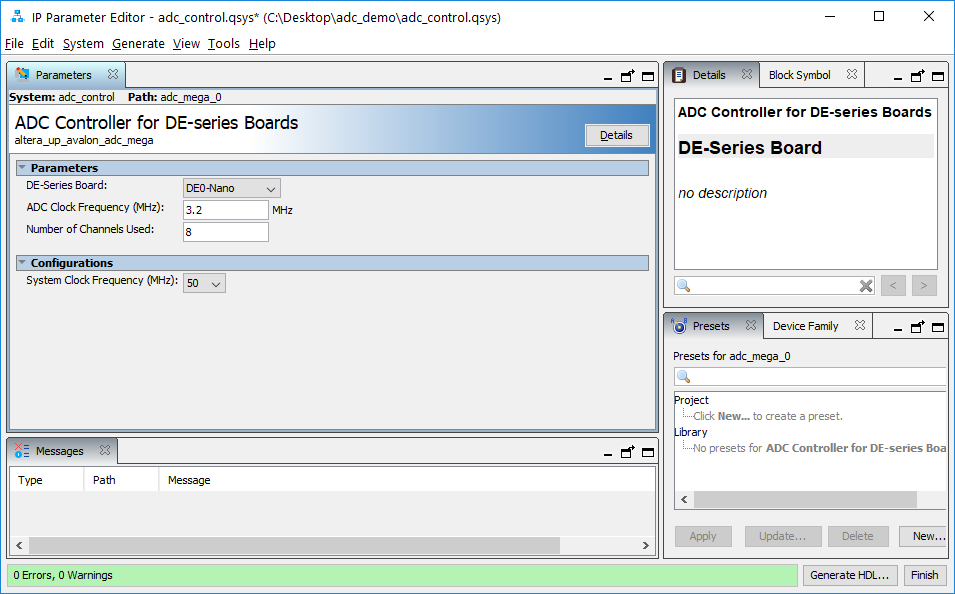
\includegraphics [scale = 0.6] {figures/ipcatalog3.png}
\end {center}
\caption {Generating the ADC controller.}
\label {fig:ipcatalog3}
\end {figure}

\begin {figure} [H]
\begin {center}
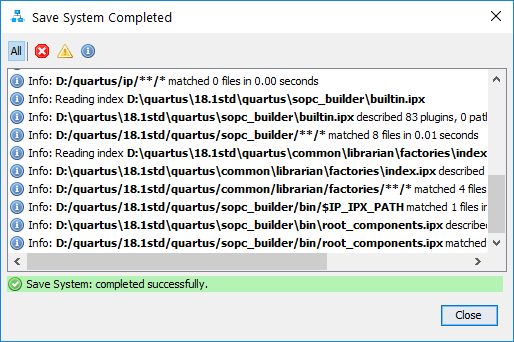
\includegraphics [scale = 0.5] {figures/ipcatalog4.png}
\end {center}
\caption {Saving the Platform Designer system for IP variation.}
\label {fig:ipcatalog4}
\end {figure}

After finishing generating the system, add the IP core to the Quartus project by including the .qip file under $<$generation\_directory$>$/synthesis folder.
%When prompted to add the Quartus II IP file to the project, click {\sf Yes}. If this dialog does not appear, the \mbox{Quartus II} IP File {\it (adc\_top.qip)} should be added manually by selecting {\sf %Project > Add/Remove Files In Project} from the main Quartus II window. \\
Once generation is complete, create a top-level file using the verilog code in Figure~\ref{fig:mega_top}, or use the file \textit{adc\_demo\_mega.v} in the ``design files'' directory. In this example, the Switches on the board are used to select the channel to display, from 0 to 7. The eight highest bits of the chosen channel are displayed on the LEDs. \\
\newpage
\begin{figure} [H]
	\lstinputlisting[language=Verilog, xleftmargin=4cm]{design_files/adc_demo_mega.v}
	\caption{Example top-level module for a project using the ADC Controller with IP Catalog.}
	\label{fig:mega_top}
\end{figure}

Import the pin settings file corresponding to your board; it can be found on the Intel FPGA University program website. Open the assignment editor and delete the entry for Current Strength as shown in Figure~\ref{fig:assign_editor}; this must be done when compiling projects containing the ADC controller plugin. Compile the project and download it to the board.

\begin{figure} [H]
\begin{center}
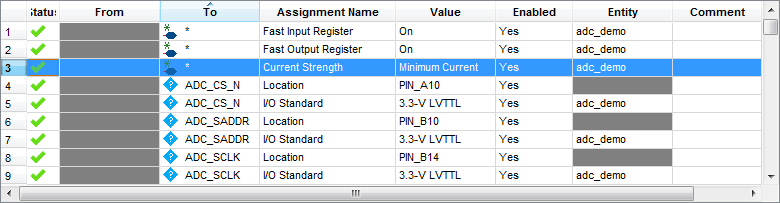
\includegraphics [scale = 0.5] {figures/assignment_editor.png}
\end {center}
\caption{Modifying Assignment Editor Entry for Current Strength}
\label{fig:assign_editor}
\end{figure}


% Copyright and Trademark

%\newcommand{\datePublished}{Mar 2022}

\newcommand{\versnum}{21.1} %version number quartus/AMP
\newcommand{\quartusname}{Quartus\textsuperscript{\textregistered} Prime}	
\newcommand{\textBar}{For \quartusname{} \versnum{}}
\newcommand{\thisyear}{2022 } %for copyright
\newcommand{\company}{FPGAcademy.org}
\newcommand{\longteamname}{FPGAcademy.org}
\newcommand{\teamname}{FPGAcademy}
\newcommand{\website}{FPGAcademy.org}

\newcommand{\productAcronym}{AMP}
\newcommand{\productNameShort}{Monitor Program}

\newcommand{\productNameMedTM}{Monitor Program}
\newcommand{\productNameMed}{Monitor Program}

%\newcommand{\headerLogoFilePath}[1]{#1/FPGAcademy.png}



%%%%%%%%%%%%%%%%%%%%%%%%%%%%%%%%%%%%%%%%
%%% FPGAcademy Copyright Information %%%
%%%%%%%%%%%%%%%%%%%%%%%%%%%%%%%%%%%%%%%%

%Always put the copyright on a new page (clear page), with some vertical space from top
\clearpage
\vspace{1in}

\noindent

Copyright {\copyright} FPGAcademy.org. All rights reserved. FPGAcademy and the FPGAcademy logo are trademarks of  FPGAcademy.org.  This document is being provided on an ``as-is'' basis and as an accommodation and therefore all warranties, representations or guarantees of any kind (whether express, implied or statutory) including, without limitation, warranties of merchantability, non-infringement, or fitness for a particular purpose, are specifically disclaimed.

%FPGAcademy assumes no responsibility or liability arising out of the application or use of any information,  product,  or  service  described  herein  except  as  expressly  agreed  to  in  writing  by  FPGAcademy.



**Other names and brands may be claimed as the property of others.




\end{document}

